\begin{tikzpicture}
%\node[minimum width=15cm,minimum height=9cm] (current page) {};
\begin{scope}[spy scope]

\node[overlay,anchor=north west,inner sep=0mm] (base) at (0, 0) {%
\only<1-2>{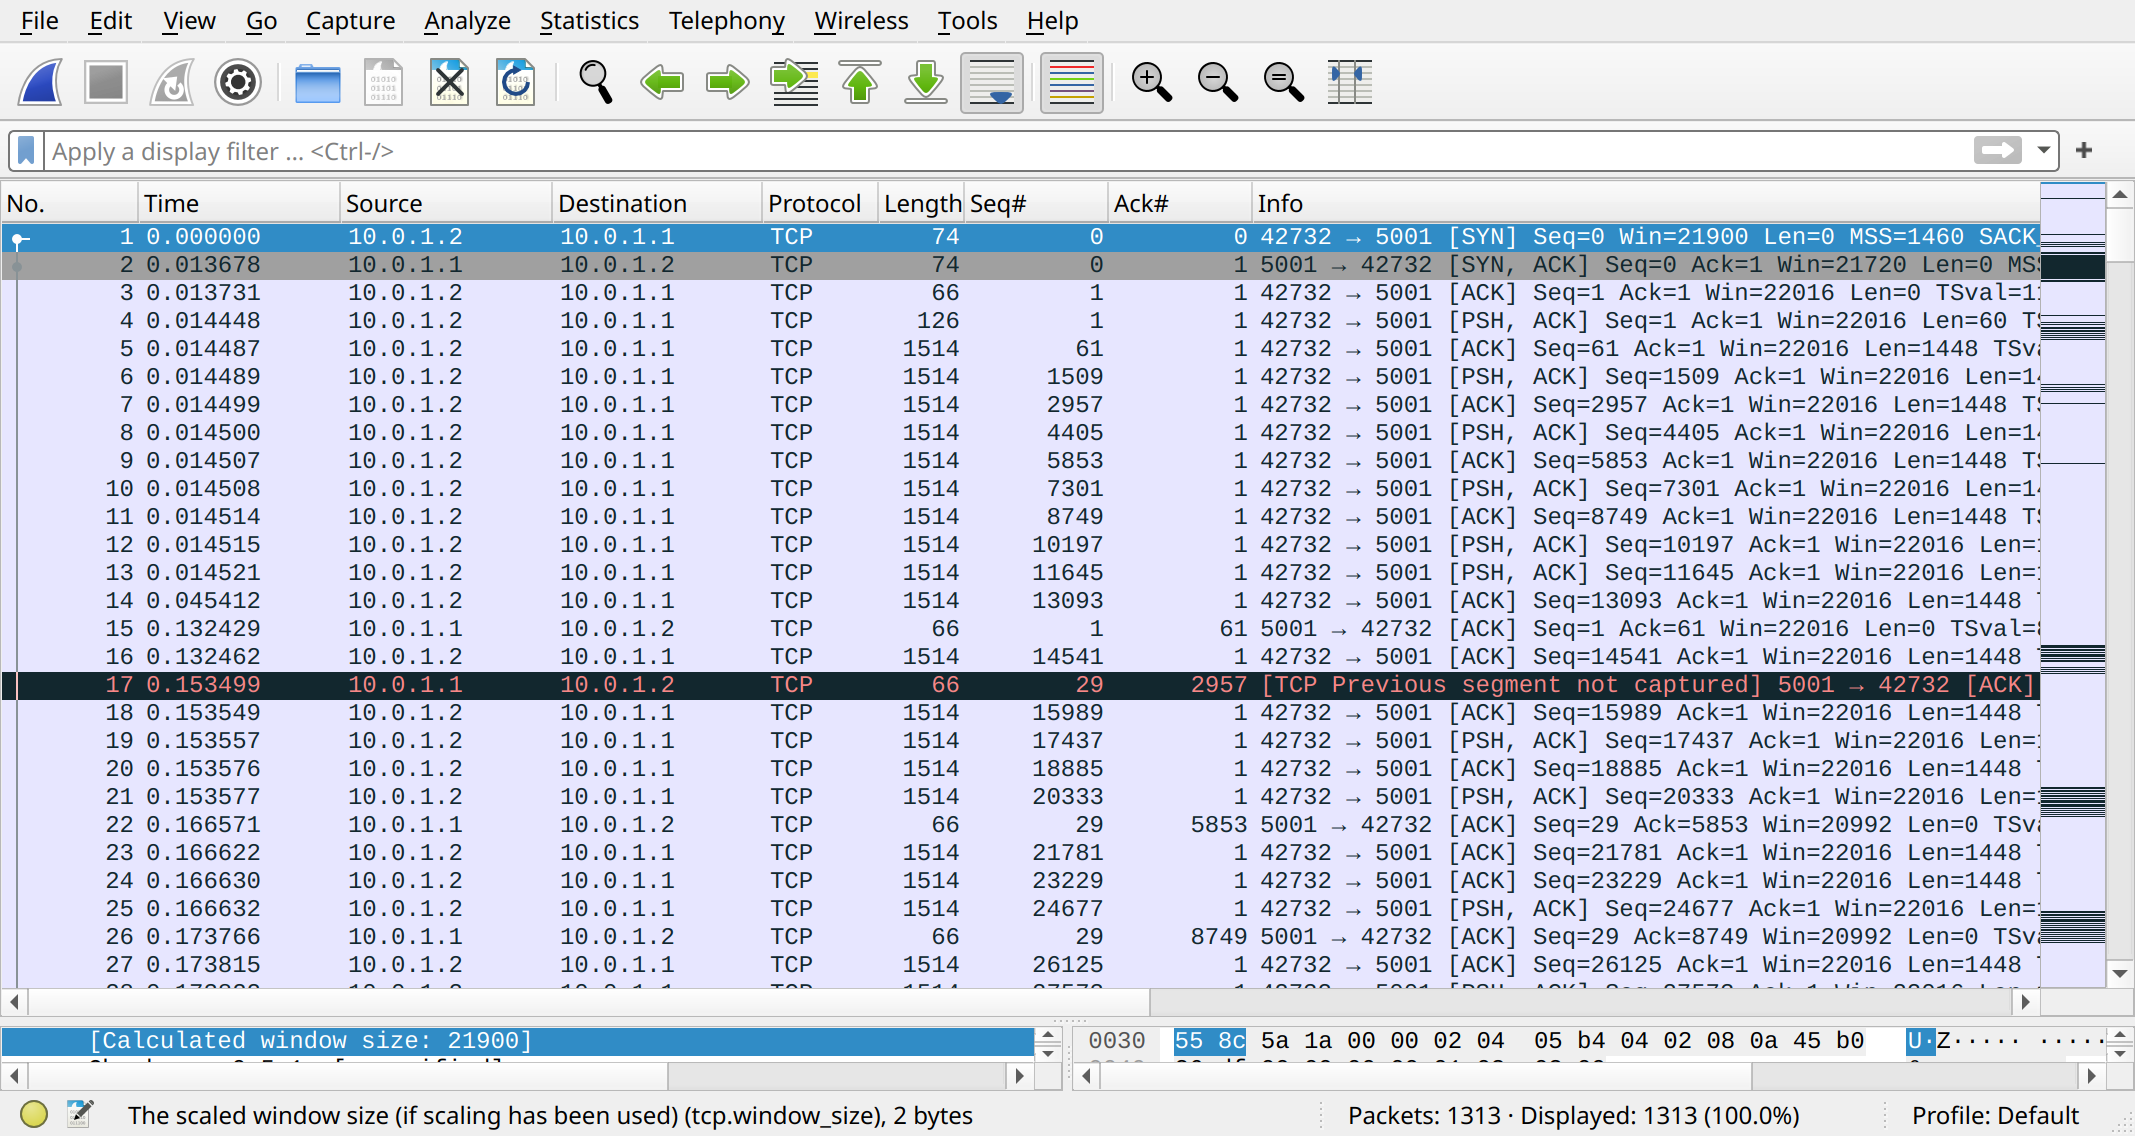
\includegraphics[width=\mypaperwidth]{../reliable/wireshark-tcp-ex2-over}}%
\only<3->{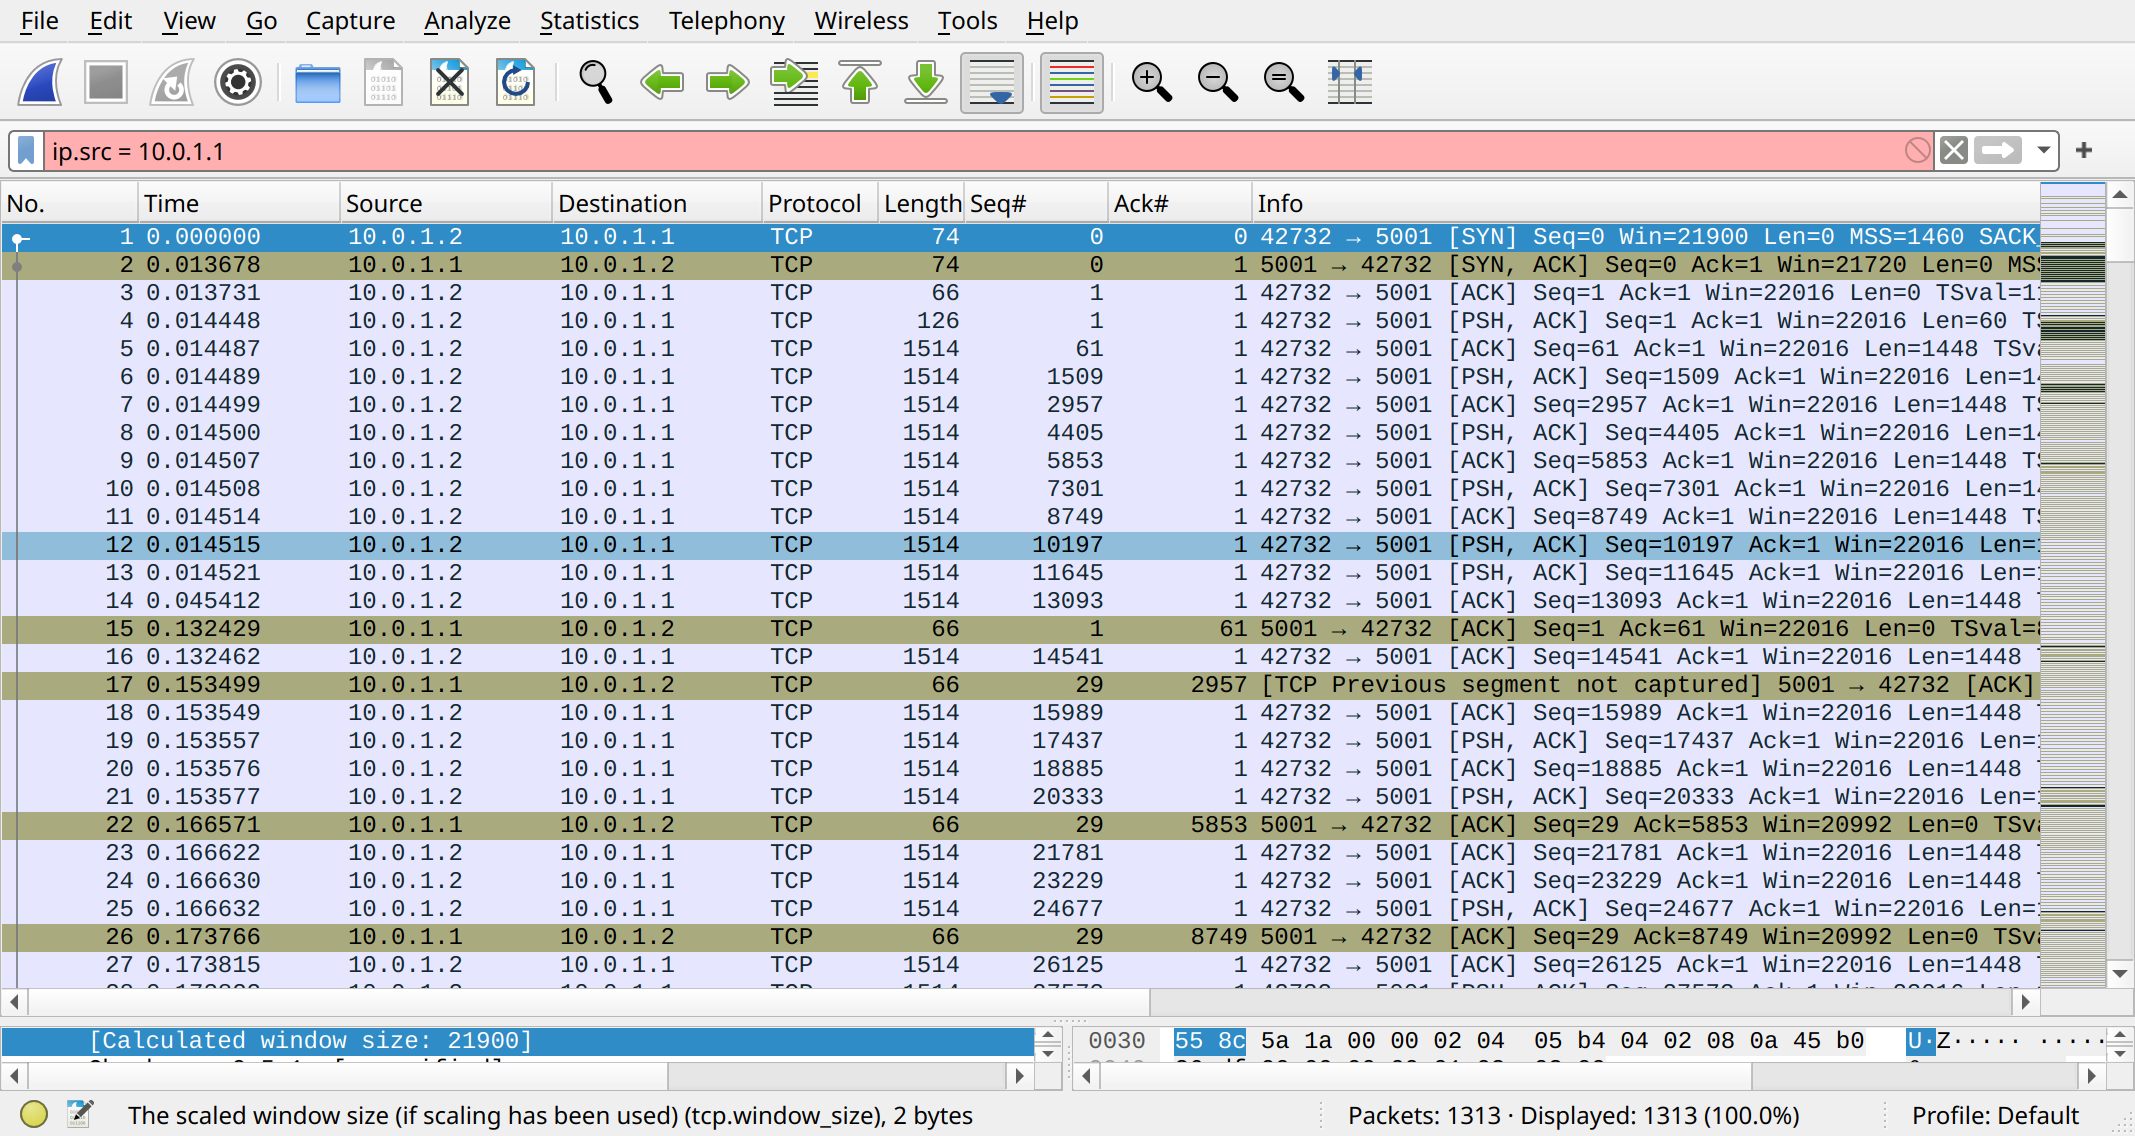
\includegraphics[width=\mypaperwidth]{../reliable/wireshark-tcp-ex2-hi-dir}}%
};
\path (0, 0) rectangle (14.5, -7); % for bounding box
%\draw[overlay,help lines] (0, 0) grid (14, -8);
%\draw[overlay,help lines,dotted] (0, 0) grid[step=0.2] (14, -8);
\begin{visibleenv}<2-3>
\path[draw,red,very thick] (0, -1.5) rectangle (13.9, -2.125);
\node[red,overlay box,anchor=north,align=left] (c setup) at (6.95, -2.125) {
    connection setup, no data transferred 
};
\end{visibleenv}
\only<3>{\spy[rectangle,width=5cm,height=2.5cm,magnification=2] on (7.45, -1.7) in node at (12, 0);}
\begin{visibleenv}<3>
\node[overlay,overlay box,font=\small,anchor=east,align=left] at (9.5, -.5) {
    server+client sequence numbers \\
    advance by 1 to indicate where in setup
};
\end{visibleenv}
\begin{visibleenv}<4>
\path[draw,red,very thick] (0, -1.7) rectangle (13.9, -1.9);
\path[draw,red,very thick] (0, -4.2) rectangle (13.9, -4.39);
\path[draw,red,very thick] (0, -4.55) rectangle (13.9, -4.75);
\path[draw,red,very thick] (0, -5.5) rectangle (13.9, -5.75);
\path[draw,red,very thick] (0, -6.25) rectangle (13.9, -6.45);
\node[overlay box,align=left,anchor=north] at (6.95, -2.5) {
    connection is bidirectional \\
    from now, using olive color to show `backwards' packets
};
\end{visibleenv}
\only<5-6>{\spy on (7.25, -2.3) in node at (10, -1);}
\only<5-6>{\spy on (8, -4.3) in node at (12, -6);}
\begin{visibleenv}<5-6>
\path[draw,red,very thick] (6.55, -2.25 + .2) rectangle (7.5, -2.45 + .2);
    \node[overlay box,text=red,anchor=east,align=left] at (6.55, -2.35) {
        data packet with \\
        client bytes 1--60
    };
\path[draw,red,very thick] (7.55, -4.2) rectangle (8.5, -4.4);
    \node[overlay box,text=red,anchor=east,align=left] at (6.55, -4.3) {
        acknowledgement of \\
        client bytes up to 60
    };
\end{visibleenv}
\begin{visibleenv}<6>
\path[draw,red,very thick] (0, -2.25) rectangle (1.9, -2.45);
\path[draw,red,very thick] (0, -4.2) rectangle (1.9, -4.4);
\path[draw,red,dotted,double,ultra thick] (1, -2.45 +.2) -- (1, -4.2) node[midway,font=\small,fill=white,fill opacity=0.957,text=red,text opacity=1.0] {118 ms};
\end{visibleenv}
\begin{visibleenv}<7>
\path[draw,red,very thick] (12.6, -4.15) rectangle (13.3, -4.4);
\path[draw,red,very thick] (6.55, -4.2) rectangle (7.55, -4.4);
\path[draw,red,very thick] (6.55, -4.55) rectangle (7.55, -4.75);
\path[draw,red,very thick] (8.5, -4.55) rectangle (12, -4.75);
\only<7>{\spy[rectangle,width=10cm,magnification=1.5,height=1cm] on (10, -4.5) in node;}
    \node[overlay box,text=red,anchor=south,align=left] at (6.55, -3.7) {
        jumps from server byte 0 to server byte 28 \\
        with no data sent \\
        wireshark IDs as missing packet
    };
% FIXME:  hilite len =0 and seq # 29
% FIXME: note missing data packet with bytes 1--28
% FIXME: screenshot scrolled down showing that
\end{visibleenv}
\end{scope}
\end{tikzpicture}
